% Chapter 8

\chapter{Artefact Design} % Main chapter title

\label{Chapter8_artefact-design} % For referencing the chapter elsewhere, use \ref{Chapter7} 

\section{Introduction }
This chapter is about the designing of the prototype artefact Cybernewsfeed Technology using Design Science Research (DSR) 
\citep{hevner2010design}. 
The research method used for this specific piece of thesis work is Creative Process 
\citep{march1995design}  
as mentioned in chapter  
\ref{Chapter6_research-approach} 
(section \ref{Research Methodology: Design Science Research}). The artefact  has been termed as \enquote{Cybernewsfeed Technology} and this chapter provides a detailed explanation on the requirement and the final design of the \enquote{Cybernewsfeed Technology}.

\section{Requirement Specification}
%%% This file contains only a table.
%% this file is included into Chapter8

\begin{table}[htbp!]
   \setlength{\arrayrulewidth}{0.2mm}
    \setlength{\tabcolsep}{5pt}
    \renewcommand{\arraystretch}{1.0}

    \centering{}
 
    \caption{Requirements Modules}
    \label{table:Modules}
    
    \begin{tabularx}{0.92\linewidth}{|X| X|X|X|X|X|} 
    
%    |a|>{\columncolor[HTML]{FFFFFF}}C|C|C|
     \arrayrulecolor[HTML]{06000A}
        %% Table Body
       
        \hline
         \rowcolor[HTML]{BFCEED} \textbf{Modules-->}	&	\textbf{Collector}	&	\textbf{Processor}	&	\textbf{Analyser}	&	\textbf{Advisor}\\
        \hline
        \rowcolor[HTML]{EAEAFC}  Processes--> &	Collection &	Processing &	Analysis &	Advisory  \\
        \hline
       
       \rowcolor[HTML]{F6F6FB} Activities--> &	Collect, Source Management & Filtering, Contexting, Tagging, Data Manipulation and Output &	Provide Insight on tactics, severity and Impact &	Advice to Customer, Simple Writeup, Publishing                                  \\
       
        \hline
    \end{tabularx}

\end{table}











%\setlength{\arrayrulewidth}{0.5mm}
%\setlength{\tabcolsep}{10pt}
%\renewcommand{\arraystretch}{1.5}

%\newcolumntype{s}{>{\columncolor[HTML]{DDBDF7}} p{3cm}}


%\begin{tabular}{ |a | >{\columncolor[HTML]{5993C2}}c | l | b }

% \arrayrulecolor[HTML]{06000A}
% \hline
% \rowcolor[HTML]{5789F3} \multicolumn{4}{|c|}{High Level Modules = Collector} \\
% \hline
%  
%  \rowcolor[HTML]{BFCEED} Requirements: & What? & Why? & MoSCoW priority \\
% \hline
%
%Language Support	 & 	Support various languages.	 & 	To not miss intel in other languages	 & 	Must have	\\
% \hline
%Data Formats	 & 	Allow multiple data formats	 & 	To collect and process standard and recent formats	 & 	Should have	\\
% \hline
%Data Source types	 & 	Ingest from various sources	 & 	To cover broader sources of Intel	 & 	Must have	\\
% \hline
%Connection protocol	 & 	Support common protocols	 & 	To allow actual transfer To data	 & 	Must have	\\
 % 
%  \hline
% \end{tabular}
 



\subsection{Approach}

 To understand the requirements, my first step was to get familiar with the existing system, processes, activities and tools used in cyber newsfeeds publication. I took two simultaneous approaches: 1) searching knowledge in literature\footnote{According to literature review in chapter \ref{Chapter7_literature-review} } and 2) getting acquainted in a pragmatic way by working together with ON2IT team\footnote{Research and Development team, ON2IT Cybersecurity, The Nederlands}. The knowledge gained in the literature review was applied to the pragmatic approach where I was collaborating directly with the ON2IT team.
 
After understanding the processes and activities, I myself as an user\footnote{Role of Cyber Analyst for a certain period} started to work on the following four activities: 1) To manual scan of the cyber newsfeed sources,  2) To collect the cyber newsfeeds, 3) To analyse the newsfeeds and 4) To prepare advisory. Working with ON2IT team as an user helped me to understand the end-to-end flow of cyber newsfeeds publication.

Another step taken to enhance my understanding was simulating the existing system into a cloud environment. I choose a cloud environment to deploy, as it was easy to deploy and easy to collaborate as compared to my personal system. 
Simulation helped me to observe and understand the behaviour of the existing system used by the cyber experts. 
I also understood the way practitioners explore the sources to find relevant cyber newsfeed items. 


\subsection{Requirement Findings}
After two months of regular interactions with the ON2IT research and development team, it helped me to outline the requirements of the Artefact. 
Then the requirements were logically grouped based on the nature of activities as shown in FIGURE \ref{fig:modules}. I have termed
the list of such activities based groups as \enquote{High level Modules}. The name of modules classified as \enquote{High level Modules} are: 1) Collector, 2) Processor, 3) Analyser and 4) Advisor.  Based on the interactions from ON2IT team, I have elaborates on the requirements of each \enquote{High level Modules} in the following sections. 

\begin{figure}[ht]
    \centering
     
    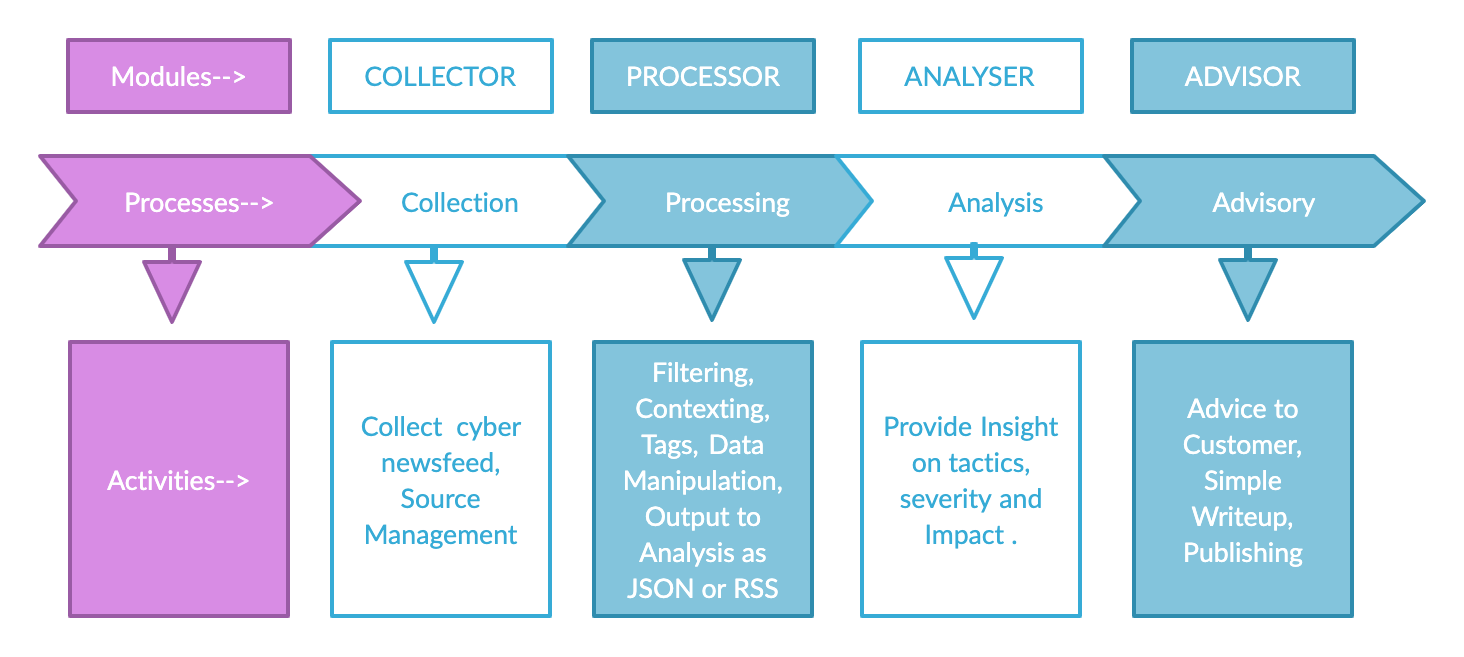
\includegraphics[width=1\linewidth]{Figures/Modules.png}
     
    \caption{Modules.
    \label{fig:modules}}
  
\end{figure}
\begin{enumerate}

    \item \textbf{Collector:}
    Collector helps to collect data from various cyber newsfeed sources and is an essential module required to proceed with the further activities of cyber newsfeed publication. 
    Collector enables to store the cyber newsfeed raw data in a repository. From this repository, the cyber newsfeed data can be assessed for further processing by the Processor module. 
    The  TABLE in \ref{table:collector-req} shows four essential requirements for the Collector module. 
    Along with requirement the reasoning is also mentioned with the priority.
%%% This file contains only a table.
%% this file is included into Chapter8

\begin{table}[htbp!]
   \setlength{\arrayrulewidth}{0.1mm}
    \setlength{\tabcolsep}{5pt}
    \renewcommand{\arraystretch}{1.0}

    \centering{}
 
    \caption{Requirements: Cyber data collection}
    \label{table:collector-req}
    
    \begin{tabularx}{0.92\linewidth}{|>{\columncolor[HTML]{ECB4E8}} p{2.2cm}|p{3.0cm}|p{4.4cm}|p{2cm}|} 
    
%    |a|>{\columncolor[HTML]{FFFFFF}}C|C|C|
     \arrayrulecolor[HTML]{06000A}
        %% Table Body
        \hline
        \rowcolor[HTML]{5789F3} 
        \multicolumn{4}{|c|}{High Level Modules = Collector} \\
        \hline
         \rowcolor[HTML]{BFCEED} Requirements: & What? & Why? & MoSCoW priority \\
        \hline
        Language Support	                    & 	
        Support various languages.	            & 	
        To not miss intel in other languages	& 	
        Must have	                            \\
        \hline
       
       
        Data Formats	                                    & 	
        Allow multiple data formats	                        & 	
        To collect and process standard and recent formats	& 	
        Should have	                                        \\
        \hline
       
        Data Source types	                & 	
        Ingest from various sources	        & 	
        To cover broader sources of Intel   & 	
        Must have	                        \\
       
        \hline
        Connection protocol	                & 	
        Support common protocols	        & 	
        To allow actual transfer To data	& 	
%|       \cellcolor[HTML]{AA0044}
        Must have	                        \\
       
        \hline
    \end{tabularx}

\end{table}











%\setlength{\arrayrulewidth}{0.5mm}
%\setlength{\tabcolsep}{10pt}
%\renewcommand{\arraystretch}{1.5}

%\newcolumntype{s}{>{\columncolor[HTML]{DDBDF7}} p{3cm}}


%\begin{tabular}{ |a | >{\columncolor[HTML]{5993C2}}c | l | b }

% \arrayrulecolor[HTML]{06000A}
% \hline
% \rowcolor[HTML]{5789F3} \multicolumn{4}{|c|}{High Level Modules = Collector} \\
% \hline
%  
%  \rowcolor[HTML]{BFCEED} Requirements: & What? & Why? & MoSCoW priority \\
% \hline
%
%Language Support	 & 	Support various languages.	 & 	To not miss intel in other languages	 & 	Must have	\\
% \hline
%Data Formats	 & 	Allow multiple data formats	 & 	To collect and process standard and recent formats	 & 	Should have	\\
% \hline
%Data Source types	 & 	Ingest from various sources	 & 	To cover broader sources of Intel	 & 	Must have	\\
% \hline
%Connection protocol	 & 	Support common protocols	 & 	To allow actual transfer To data	 & 	Must have	\\
 % 
%  \hline
% \end{tabular}
 

 %includes may not be nested

%% This file contains only a table.
%% this file is included into Chapter8

\begin{table}[htbp!]
   \setlength{\arrayrulewidth}{0.1mm}
    \setlength{\tabcolsep}{5pt}
    \renewcommand{\arraystretch}{1.0}

    \centering{}
 
    \caption{Requirements: Cyber data collection}
    \label{table:collector-req}
    
    \begin{tabularx}{0.92\linewidth}{|>{\columncolor[HTML]{ECB4E8}} p{2.2cm}|p{3.0cm}|p{4.4cm}|p{2cm}|} 
    
%    |a|>{\columncolor[HTML]{FFFFFF}}C|C|C|
     \arrayrulecolor[HTML]{06000A}
        %% Table Body
        \hline
        \rowcolor[HTML]{5789F3} 
        \multicolumn{4}{|c|}{High Level Modules = Collector} \\
        \hline
         \rowcolor[HTML]{BFCEED} Requirements: & What? & Why? & MoSCoW priority \\
        \hline
        Language Support	                    & 	
        Support various languages.	            & 	
        To not miss intel in other languages	& 	
        Must have	                            \\
        \hline
       
       
        Data Formats	                                    & 	
        Allow multiple data formats	                        & 	
        To collect and process standard and recent formats	& 	
        Should have	                                        \\
        \hline
       
        Data Source types	                & 	
        Ingest from various sources	        & 	
        To cover broader sources of Intel   & 	
        Must have	                        \\
       
        \hline
        Connection protocol	                & 	
        Support common protocols	        & 	
        To allow actual transfer To data	& 	
%|       \cellcolor[HTML]{AA0044}
        Must have	                        \\
       
        \hline
    \end{tabularx}

\end{table}











%\setlength{\arrayrulewidth}{0.5mm}
%\setlength{\tabcolsep}{10pt}
%\renewcommand{\arraystretch}{1.5}

%\newcolumntype{s}{>{\columncolor[HTML]{DDBDF7}} p{3cm}}


%\begin{tabular}{ |a | >{\columncolor[HTML]{5993C2}}c | l | b }

% \arrayrulecolor[HTML]{06000A}
% \hline
% \rowcolor[HTML]{5789F3} \multicolumn{4}{|c|}{High Level Modules = Collector} \\
% \hline
%  
%  \rowcolor[HTML]{BFCEED} Requirements: & What? & Why? & MoSCoW priority \\
% \hline
%
%Language Support	 & 	Support various languages.	 & 	To not miss intel in other languages	 & 	Must have	\\
% \hline
%Data Formats	 & 	Allow multiple data formats	 & 	To collect and process standard and recent formats	 & 	Should have	\\
% \hline
%Data Source types	 & 	Ingest from various sources	 & 	To cover broader sources of Intel	 & 	Must have	\\
% \hline
%Connection protocol	 & 	Support common protocols	 & 	To allow actual transfer To data	 & 	Must have	\\
 % 
%  \hline
% \end{tabular}
 



    \item \textbf{Processor:}
     Processor module would be responsible for cyber newsfeed data filtering, manipulation and tagging.
     The data filtering manipulation and tagging methods should support filtration, manipulation and tagging based on the configurable parameters. 
     The Processor module must verify the content of the configured tags and must add a tag to the cyber newsfeed data based on the input parameters. 
     The input parameters could be stakeholders specific or an organisation specific.
     The TABLE \ref{table:processor-req} contains the list of requirements for the Processor module.
    
%% This file contains only a table.
%% this file is included into Chapter8

\begin{table}[htbp!]
   \setlength{\arrayrulewidth}{0.1mm}
    \setlength{\tabcolsep}{5pt}
    \renewcommand{\arraystretch}{1.0}

    \centering{}
 
    \caption{Requirements: Cyber data processing}
    \label{table:processor-req}
    
    \begin{tabularx}{0.92\linewidth}{|>{\columncolor[HTML]{ECB4E8}} p{2.2cm}|p{3.0cm}|p{4.4cm}|p{2cm}|} 
    
%    |a|>{\columncolor[HTML]{FFFFFF}}C|C|C|
     \arrayrulecolor[HTML]{06000A}
        %% Table Body
        \hline
        \rowcolor[HTML]{5789F3} 
        \multicolumn{4}{|c|}{High Level Module = Processor} \\
        \hline
         \rowcolor[HTML]{BFCEED} Requirements: & What? & Why? & MoSCoW priority \\
        \hline
      Data structuring	 & 	Data mappings and Data format conversion	 & 	To ensure a common data format To enable further processing	 & 	Should have	\\
       \hline
Contextualiz-ation	 & 	Possible to set context	 & 	To convert raw intel To specific intel	 & 	Must have	\\
       
        \hline
Data Filtering	 & 	Be able to filter data 	 & 	Based on adjustable parameters	 & 	Must have	\\
       
        \hline
    \end{tabularx}

\end{table}











%\setlength{\arrayrulewidth}{0.5mm}
%\setlength{\tabcolsep}{10pt}
%\renewcommand{\arraystretch}{1.5}

%\newcolumntype{s}{>{\columncolor[HTML]{DDBDF7}} p{3cm}}


%\begin{tabular}{ |a | >{\columncolor[HTML]{5993C2}}c | l | b }

% \arrayrulecolor[HTML]{06000A}
% \hline
% \rowcolor[HTML]{5789F3} \multicolumn{4}{|c|}{High Level Modules = Collector} \\
% \hline
%  
%  \rowcolor[HTML]{BFCEED} Requirements: & What? & Why? & MoSCoW priority \\
% \hline
%
%Language Support	 & 	Support various languages.	 & 	To not miss intel in other languages	 & 	Must have	\\
% \hline
%Data Formats	 & 	Allow multiple data formats	 & 	To collect and process standard and recent formats	 & 	Should have	\\
% \hline
%Data Source types	 & 	Ingest from various sources	 & 	To cover broader sources of Intel	 & 	Must have	\\
% \hline
%Connection protocol	 & 	Support common protocols	 & 	To allow actual transfer To data	 & 	Must have	\\
 % 
%  \hline
% \end{tabular}
 


    
%%% This file contains only a table.
%% this file is included into Chapter8

\begin{table}[htbp!]
   \setlength{\arrayrulewidth}{0.1mm}
    \setlength{\tabcolsep}{5pt}
    \renewcommand{\arraystretch}{1.0}

    \centering{}
 
    \caption{Requirements: Cyber data collection}
    \label{table:collector-req}
    
    \begin{tabularx}{0.92\linewidth}{|>{\columncolor[HTML]{ECB4E8}} p{2.2cm}|p{3.0cm}|p{4.4cm}|p{2cm}|} 
    
%    |a|>{\columncolor[HTML]{FFFFFF}}C|C|C|
     \arrayrulecolor[HTML]{06000A}
        %% Table Body
        \hline
        \rowcolor[HTML]{5789F3} 
        \multicolumn{4}{|c|}{High Level Modules = Collector} \\
        \hline
         \rowcolor[HTML]{BFCEED} Requirements: & What? & Why? & MoSCoW priority \\
        \hline
        Language Support	                    & 	
        Support various languages.	            & 	
        To not miss intel in other languages	& 	
        Must have	                            \\
        \hline
       
       
        Data Formats	                                    & 	
        Allow multiple data formats	                        & 	
        To collect and process standard and recent formats	& 	
        Should have	                                        \\
        \hline
       
        Data Source types	                & 	
        Ingest from various sources	        & 	
        To cover broader sources of Intel   & 	
        Must have	                        \\
       
        \hline
        Connection protocol	                & 	
        Support common protocols	        & 	
        To allow actual transfer To data	& 	
%|       \cellcolor[HTML]{AA0044}
        Must have	                        \\
       
        \hline
    \end{tabularx}

\end{table}











%\setlength{\arrayrulewidth}{0.5mm}
%\setlength{\tabcolsep}{10pt}
%\renewcommand{\arraystretch}{1.5}

%\newcolumntype{s}{>{\columncolor[HTML]{DDBDF7}} p{3cm}}


%\begin{tabular}{ |a | >{\columncolor[HTML]{5993C2}}c | l | b }

% \arrayrulecolor[HTML]{06000A}
% \hline
% \rowcolor[HTML]{5789F3} \multicolumn{4}{|c|}{High Level Modules = Collector} \\
% \hline
%  
%  \rowcolor[HTML]{BFCEED} Requirements: & What? & Why? & MoSCoW priority \\
% \hline
%
%Language Support	 & 	Support various languages.	 & 	To not miss intel in other languages	 & 	Must have	\\
% \hline
%Data Formats	 & 	Allow multiple data formats	 & 	To collect and process standard and recent formats	 & 	Should have	\\
% \hline
%Data Source types	 & 	Ingest from various sources	 & 	To cover broader sources of Intel	 & 	Must have	\\
% \hline
%Connection protocol	 & 	Support common protocols	 & 	To allow actual transfer To data	 & 	Must have	\\
 % 
%  \hline
% \end{tabular}
 

 %includes may not be nested

    \item \textbf{Analyzer:}
    The Analyser module is required for correlation and analysis on the cyber newsfeed data processed by the Processor module. 
    The correlation and analysis activities would be done manually by the cyber experts in the first version of the artefact. The artefact should provide a GUI to conduct analysis and correlation activities. The detailed requirements of this module is in TABLE \ref{table:analyzer-req}
    %% This file contains only a table.
%% this file is included into Chapter8

\begin{table}[htbp!]
   \setlength{\arrayrulewidth}{0.1mm}
    \setlength{\tabcolsep}{5pt}
    \renewcommand{\arraystretch}{1.0}

    \centering{}
 
    \caption{Requirements: Cyber data analysis}
    \label{table:analyzer-req}
    
    \begin{tabularx}{0.92\linewidth}{|>{\columncolor[HTML]{ECB4E8}} p{2.2cm}|p{3.0cm}|p{4.4cm}|p{2cm}|} 
    
%    |a|>{\columncolor[HTML]{FFFFFF}}C|C|C|
     \arrayrulecolor[HTML]{06000A}
        %% Table Body
        \hline
        \rowcolor[HTML]{5789F3} 
        \multicolumn{4}{|c|}{High Level Module = Analyser} \\
        \hline
         \rowcolor[HTML]{BFCEED} Requirements: & What? & Why? & MoSCoW priority \\
        \hline
     Co-relation	 & 	Group similar Intel	 & 	To reduce duplicity and improve granularity	 & 	Should have	\\
      \hline
Analysis	 & 	Provide insights on tactics, severity and impact	 & 	To make the cyber intel actionable	 & 	Must have	\\
       
        \hline
    \end{tabularx}

\end{table}











%\setlength{\arrayrulewidth}{0.5mm}
%\setlength{\tabcolsep}{10pt}
%\renewcommand{\arraystretch}{1.5}

%\newcolumntype{s}{>{\columncolor[HTML]{DDBDF7}} p{3cm}}


%\begin{tabular}{ |a | >{\columncolor[HTML]{5993C2}}c | l | b }

% \arrayrulecolor[HTML]{06000A}
% \hline
% \rowcolor[HTML]{5789F3} \multicolumn{4}{|c|}{High Level Modules = Collector} \\
% \hline
%  
%  \rowcolor[HTML]{BFCEED} Requirements: & What? & Why? & MoSCoW priority \\
% \hline
%
%Language Support	 & 	Support various languages.	 & 	To not miss intel in other languages	 & 	Must have	\\
% \hline
%Data Formats	 & 	Allow multiple data formats	 & 	To collect and process standard and recent formats	 & 	Should have	\\
% \hline
%Data Source types	 & 	Ingest from various sources	 & 	To cover broader sources of Intel	 & 	Must have	\\
% \hline
%Connection protocol	 & 	Support common protocols	 & 	To allow actual transfer To data	 & 	Must have	\\
 % 
%  \hline
% \end{tabular}
 

.

    \item \textbf{Advisory:}
    The requirement for this module is help cyber analyst in drafting a nice list of cyber newsfeed advisory. The Advisory module should ship the outbound communication to the stakeholders, via a certain communication channel. If possible, the Advisory module should also collect the feedback from users. The exact requirements of the Advisory module are listed in the %% This file contains only a table.
%% this file is included into Chapter8

\begin{table}[htbp!]
   \setlength{\arrayrulewidth}{0.1mm}
    \setlength{\tabcolsep}{5pt}
    \renewcommand{\arraystretch}{1.0}

    \centering{}
 
    \caption{Requirements: Cyber Intel advisory}
    \label{table:advisory-req}
    
    \begin{tabularx}{0.92\linewidth}{|>{\columncolor[HTML]{ECB4E8}} p{2.2cm}|p{3.0cm}|p{4.4cm}|p{2cm}|} 
    
%    |a|>{\columncolor[HTML]{FFFFFF}}C|C|C|
     \arrayrulecolor[HTML]{06000A}
        %% Table Body
        \hline
        \rowcolor[HTML]{5789F3} 
        \multicolumn{4}{|c|}{High Level Module = Advisory} \\
        \hline
         \rowcolor[HTML]{BFCEED} Requirements: & What? & Why? & MoSCoW priority \\
        \hline
     Writing custom intel	 & 	Allow to write a new content for cyber news feed	 & 	To ensure that analyst can use his knowledge for providing details on cyber news	 & 	Must have	\\
     \hline
Template Designing	 & 	Make design template for writing cyber intel and advisories	 & 	To allow flexibility in presentation of cyber Intel To further streams	 & 	Should have	\\
\hline
Feedback Collection	 & 	Collect internal and external user feedback	 & 	To check the quality and if the news is actionable	 & 	Could have	\\
\hline
Outbound Communication	 & 	Deliver Cyber news feed to users	 & 	To ensure cyber intel with advisory reach To destination	 & 	Must have	\\
       
        \hline
    \end{tabularx}

\end{table}











%\setlength{\arrayrulewidth}{0.5mm}
%\setlength{\tabcolsep}{10pt}
%\renewcommand{\arraystretch}{1.5}

%\newcolumntype{s}{>{\columncolor[HTML]{DDBDF7}} p{3cm}}


%\begin{tabular}{ |a | >{\columncolor[HTML]{5993C2}}c | l | b }

% \arrayrulecolor[HTML]{06000A}
% \hline
% \rowcolor[HTML]{5789F3} \multicolumn{4}{|c|}{High Level Modules = Collector} \\
% \hline
%  
%  \rowcolor[HTML]{BFCEED} Requirements: & What? & Why? & MoSCoW priority \\
% \hline
%
%Language Support	 & 	Support various languages.	 & 	To not miss intel in other languages	 & 	Must have	\\
% \hline
%Data Formats	 & 	Allow multiple data formats	 & 	To collect and process standard and recent formats	 & 	Should have	\\
% \hline
%Data Source types	 & 	Ingest from various sources	 & 	To cover broader sources of Intel	 & 	Must have	\\
% \hline
%Connection protocol	 & 	Support common protocols	 & 	To allow actual transfer To data	 & 	Must have	\\
 % 
%  \hline
% \end{tabular}
 

 TABLE \ref{table:advisory-req}.
   \FloatBarrier
\end{enumerate}

\subsection{Contribution to Stakeholder Goals}
In this section I have assumed the needs of cyber newsfeed intel for the stakeholders according to the literature. The stakeholders are positioned at different functional layers and are broadly classified into three levels 1) Strategic 2) Tactical and 3) Operational level. Stakeholders
\citep{farnham2013tools} are the users of cyber newsfeed intel and are collectively responsible for securing their organisational IT infrastructures. 

The board, which works at strategic level is interested in legal implications of a security breach. 
The tactical level is responsible for ensuring the fulfilment of strategic needs with the help of operational levels. 
For Instance, the analysis of loss and listing potential vulnerable assets would be scope of tactical level. 
The operational layer is responsible for taking steps to stop actual security incidents. 
For example, applying a secure patch. 

The stakeholders needs relevant and actionable intelligence rather than raw information
\citep{tounsi2018survey}.  
Following are certain characteristics required in the cyber newsfeed items to become an actionable cyber newsfeed. 

\begin{itemize}
    \item \textbf{Timely:} For effective threat intelligence time plays a critical role. 
    Intelligence ought to be quickly conveyed with insignificant idleness. 
    
    \item \textbf{Relevant:} 
    Threat intelligence needs to apply to the related environment. 
    \item  \textbf{Accurate:} 
    To be able to take more reasonable and effective measurements against attacks more accurate intelligence is necessary. Therefore, the information which is provided by threat intelligence should be correct, complete, and explicit. 
    
    \item \textbf{Specific:} 
    More detailed and more specific threat intelligence can allow defenders to choose suitable countermeasures.
    
    \item \textbf{Actionable}: 
    Actions are needed to be identified by threat intelligence to ensure necessary data for the response against threats.

\end{itemize}


The mapping between the concerned cyber newsfeed type and the stakeholders is shown in the FIGURE \ref{fig:stakeholder-problem}.

\begin{figure}[ht]
    \centering
     
    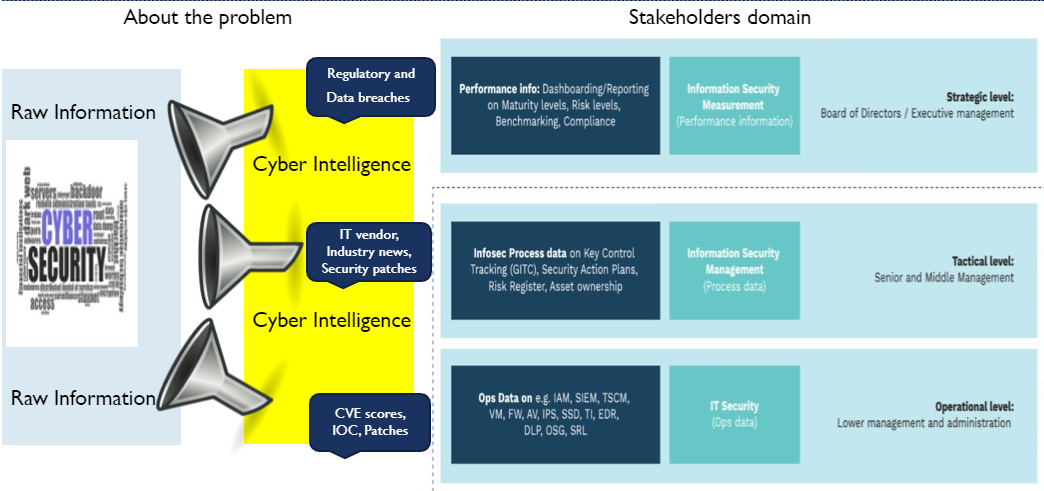
\includegraphics[width=1\linewidth]{Figures/stakeholder-problem}
     
    \caption{Stakeholders: Volumetric Problems at Three levels.
    \label{fig:stakeholder-problem}}
  
\end{figure}

According to ON2IT team, the cyber newsfeed intelligence can be analysed, classified and Tagged into one of the the levels: 1) Strategic, 2) Tactical and 3) Operational to make it interceptable at the stakeholders end. 



\begin{table}[hbt!]
    \caption{Cyber Information needs per level}
    \label{tab:stakeholder-news}
    \centering
    \resizebox{0.75\textwidth}{!}{%
        \begin{tabular}{|l|l|}
        \toprule
            \textbf{Indented news Level} & 
            \textbf{Cyber newsfeed type} \\
            \midrule
            Strategic & Regulatory News	\\
            Strategic & Data breaches - sector	\\
            Strategic/Tactical & Guidelines from community bodies (NCSC)\\
            Strategic/Tactical & Industry news\\
            Tactical/Operational & Security vendor news (new releases patches)\\
            Tactical & Market indicators and reports\\
            Operational & Important updates from tech vendors	\\
            Operational & CVE scores , Advisory, IOC , Impact	\\
            \bottomrule
        \end{tabular}
    }
\end{table}

\subsection{Available artefact}
The available artefact in practice was Taranis\footnote{About Taranis \url{https://github.com/NCSC-NL/taranis3/wiki}} at ON2IT. Other tools mentioned in the list \ref{tab:tip-list} are according to the literature. 
Taranis is used for collection and source management, 
further the filtering and selection of cyber newsfeed is a manual process. 
Although Taranis support the feature of pushing publication after advisory but it is barely used to perform such activities. 
The main reason is partial ingestion of cyber newsfeeds for any particular topic and complex data models in the Taranis database. 

There are list \ref{tab:tip-list} of tools  including Taranis  that only support parts of the functionality like collecting the cyber newsfeed data but they do not fulfill the  needs of customised data processing and relevance tagging,  therefore a new artefact was needed.

\section{New artefact prototype}\label{New artefact prototype design}
This section covers in detail about the newly created artefact:  
1) Prototype to filter contextual cyber Intelligence, perform automatic relevance tagging and perform analysis for automated risk determination and advisory and 
2)  Prototype on accessing the data source quality to keep data sources sanitized

\subsection{Prototype for, filtering contextual feeds, perform automatic tagging and analysis of risk determination and advisory.}

\subsubsection{Introduction}
This section describes the approach and work done to build the artefact. 
In the subsequent sections, there is logical segregation done based on the activities done to deliver the artefact.
It also includes the list of modules required to build the artefact where 
each artefact module is then explained in detail. 


\begin{table}
    \caption{Assessment Parameters for tool selection}
    \label{table: assessment-parameters}
    \centering{}
   \resizebox{0.75\textwidth}{!}{
    \begin{tabular}{|>{\columncolor[HTML]{ECB4E8}}l|l|}
    \toprule
      \rowcolor[HTML]{BFCEED} 
    
    \textbf{Assessment Parameters} & \textbf{Focus}\\
    \midrule
    Distribution & Open Source\\
    Application Support Forum  Available? & Ease of trouble shoot\\
    Application Active Since years & Old and stable\\
    Application's Last Issue resolved date & Most recent is better\\
    Functional Features &	More is better\\
    Database and GUI & User Friendly\\
   \bottomrule
 
    \end{tabular}
}
\end{table}

\subsubsection{Approach to build artefact}
After the process of requirement elicitation, the artefact requirements were clear and I started evaluating available threat intelligence tools based on the assessment parameters listed in table \ref{table: assessment-parameters} for the required functionality and priority. 
An ideal threat intelligence tool should provide Collector, Processor, Analyser and Advisory modules. Finding everything in one tool which is readily available in one threat intelligence tool was not possible. 
Out of 17 listed tool in \ref{tab:tip-list}, four were shortlisted as listed in table \ref{tab:four-tool}.


\begin{table}
    \caption{Shortlisted tools for cybernewfeed technology}
    \label{tab:four-tool}
    \centering{}
   \resizebox{\textwidth}{!}{
    \begin{tabular}{|>{\columncolor[HTML]{ECB4E8}}l|l|}
    \toprule
      \rowcolor[HTML]{BFCEED} 
    
    \textbf{Shortlisted Applications} & \textbf{Brief Overview}\\
    \midrule
   
FreshRSS & 
Good choice only for Collection \\
MISP: Open-source threat intelligence platform &
Used to store, share and collaborate on cyber security indicators\\
CRITs: Collaborative Research Into Threats &
CISCO will stop Grant in 2020\\
Collection Intel Framework &
Combine with machine learning to produce unified threat feeds\\

   \bottomrule
 
    \end{tabular}
}
\end{table}




We chose Fressrss from existing lists of vendors which provide newsfeed collection as open source for Collector process. This module will collect and store cyber newsfeed information in a central repository. On the top of Collector module, we  build Processor, Analyser and Advisory. We developed the functionality of data filtering, text manipulation, relevance tagging on the information stored in the central repository. We have used AWS cloud to build, deploy and run the solution because of the two reasons. 1) The cloud usage charges could be paid on hourly basis and 2) I am much familiar with AWS cloud then other cloud providers.

\subsection{Argumentation}
This section explains the logic and rationale used to choose any specific processes, activities or tools for the purpose of building the artefact. Let’s see in detail.

At general level, we had six parameters for overall evaluation of a threat intel tool. 
Those parameters are listed below with the focus area. 
We were looking for a stable
\citep{THE-BIT-DEPTH-BLOG} open source tool\footnote{Refer to defination of open source software according to Wikipedia \url{https://en.wikipedia.org/wiki/Open-source_software}} with maximum functionality and is easy to operate. 
The preference to select a stable open source tools was to save the time by reusing a stable tool and saving cost by using open source.

There were total 23 tools evaluated and four shortlisted to look into more detail. Out of these four tools, FressRss was selected because of it’s primarily capability to collect newsfeed information from different sources in a central repository and its simplicity of deployment and control on information collected. As the FreshRSS is PHP based application with MySQL as database, to process information further, it was easy to build custom modules on the top of the central repository.  

For Processor module, we developed our own configurable system because the rule required to filter, contextualize, tag and categorize is specific to stakeholder needs and does not comes with any available open source tool. Similarly, Analyser and Advisory modules are human intensive and require certain process set-up specific to the stakeholder need. Both cyber analysis and editorial tasks requires human intervention to provide essential insights. 

\subsection{Artefact and Artefact breakdown }\label{Artefact and Artefact breakdown}
\begin{figure}[ht]
    \centering
    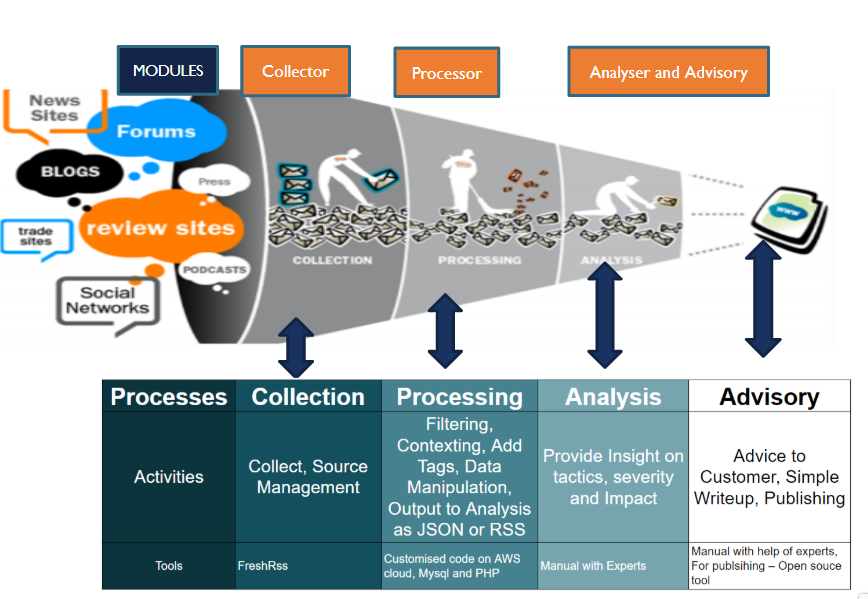
\includegraphics[width=1\linewidth,height=0.5\textwidth]{Figures/solution-breakup.PNG}
    \caption{Artefact: At a glance}
    \label{fig:solution-breakup}
\end{figure}

\subsubsection{Collector Module}
The model of the Collector module in the artefact has been depicted in FIGURE \ref{fig:collector}.
The Collector module is designed to collect cyber newsfeed from different web based data sources and source management.   
 For example, a data source \enquote{feed:\url{https://www.darkreading.com/rss_simple.asp?f_n=644&f_ln=Attacks/Breaches} }can be added as a source in the Collector module. By doing data source management, an user can add, 
remove and update the list of data sources in the Collector module.
The Collector module is  the core of the \enquote{Cybernewsfeed Technology} because this module collects and stores information for further processing. Using the Collector module, an user can collect cyber newsfeeds in other languages.
It can also collect data in real time mode as well as in batch mode as shown in FIGURE \ref{ref:collector-batch}. 
In case the Collector module has not run in last few days, the user can use batch mode to collect the backlog data. 

We have used open source tool FressRSS and installed it on AWS cloud for simulating the Collector module.

\begin{figure}[ht]
    \centering
    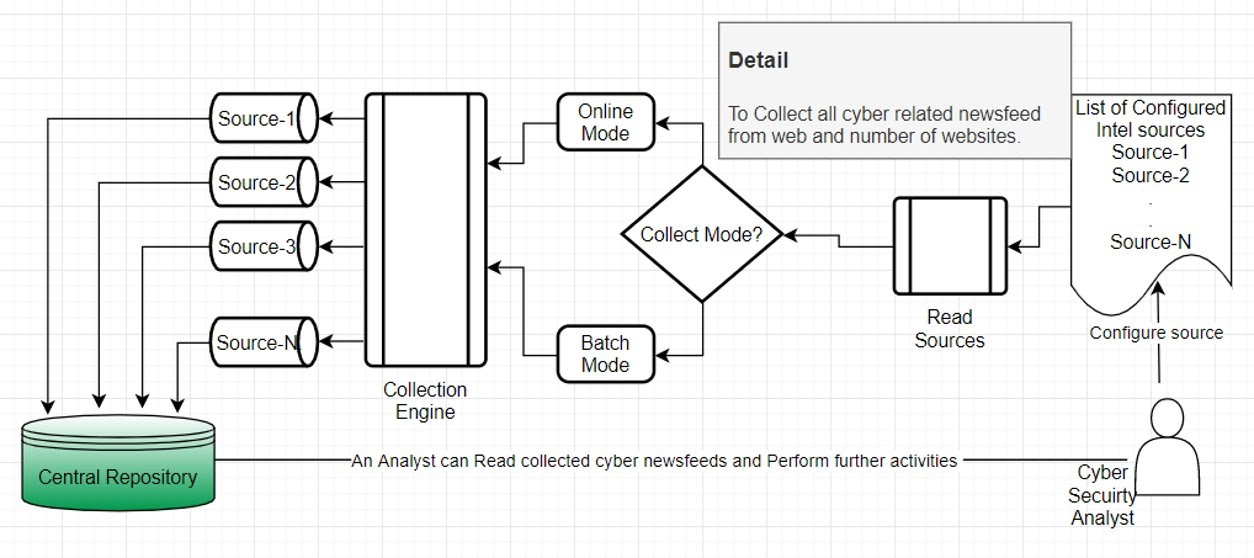
\includegraphics[width=1\linewidth]{Figures/collector.png}
    \caption{Collection Module Design}
    \label{fig:collector}
\end{figure}


\begin{figure}[ht]
\centering
    \fbox{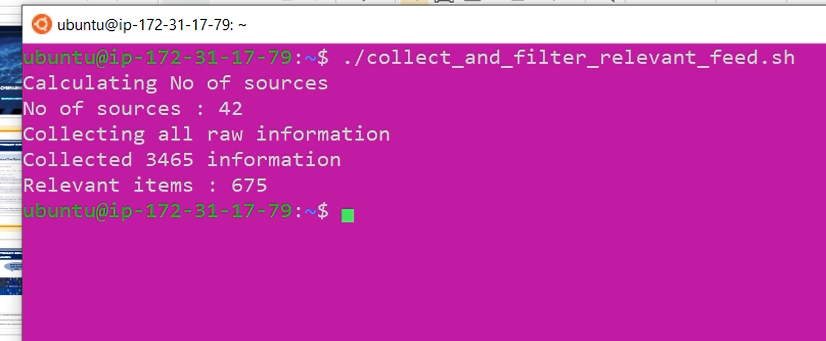
\includegraphics[width=.75\linewidth]{Figures/Collector-Demo.PNG}}
    \caption{Screenshot of the artefact: FreshRSS in Batch collection }
    \label{ref:collector-batch}
\end{figure}

In the FIGURE \ref{ref:collector-batch}, 
we see that the script invoked the batch job to collect the cyber newsfeed from 42 sources, 
it scanned and collected 3465 information and highlighted 675 relevant items.

\subsubsection{Processor Module}
The Processor module is at the heart of this cybernewsfeed technology and the model of the Processor module in the artefact has been depicted in FIGURE \ref{fig:processor}. 
\begin{figure}[ht]
    \centering
    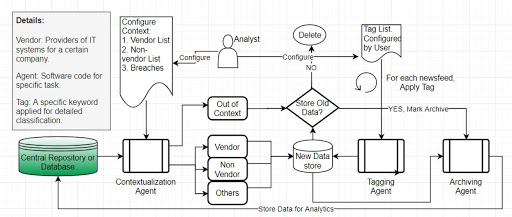
\includegraphics[width=1\linewidth]{Figures/processor.png}
    \caption{Processor Module Design}
    \label{fig:processor}
\end{figure}
 \FloatBarrier
In the Processor module, the first step is to configure the organisation-specific context by using TAGs. To configure the organisation-specific context, the Processor module needs the list of context and tags from the organisation-specific stakeholders.  A cyber security analyst can configure the organisational-specific context by use of the keywords, 
see FIGURE \ref{fig:tag} for tag management and FIGURE \ref{fig:Configured-tags} for the list of already configured tags. In this demo we have considered Vendor and Non-Vendor aspects of the context for ON2IT and TAGs like (Relevant Vendors: Cisco, Palo Alto, etc and Less relevant Vendors for ON2IT: Zoom, etc). The configured keywords in  the Processor module filters the organisation-specific cyber newsfeed according to the code mentioned in \ref{filter-context} in Appendix \ref{AppendixChapter8}.

\begin{figure}[ht]
    \centering
    \fbox{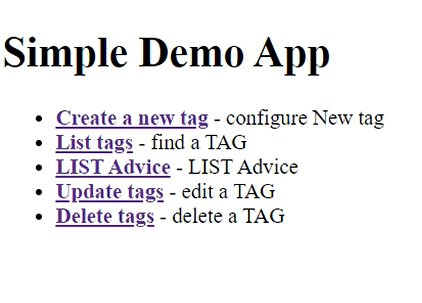
\includegraphics[width=.5\linewidth]{Figures/tag.PNG}}
    \caption{Screenshot of the artefact: Demo for TAG management}
    \label{fig:tag}
\end{figure}
 \FloatBarrier
    At the second level of processing in the Processor module, a tagging agent (software) 
tags the  cyber newsfeed with specific tags at more granular level to classify 
the news into detailed contexts, 
as specified in FIGURE \ref{tab:stakeholder-news} using code in \ref{tag-addtag} in Appendix \ref{AppendixChapter8}.

\begin{figure}[ht]
    \centering
    \fbox{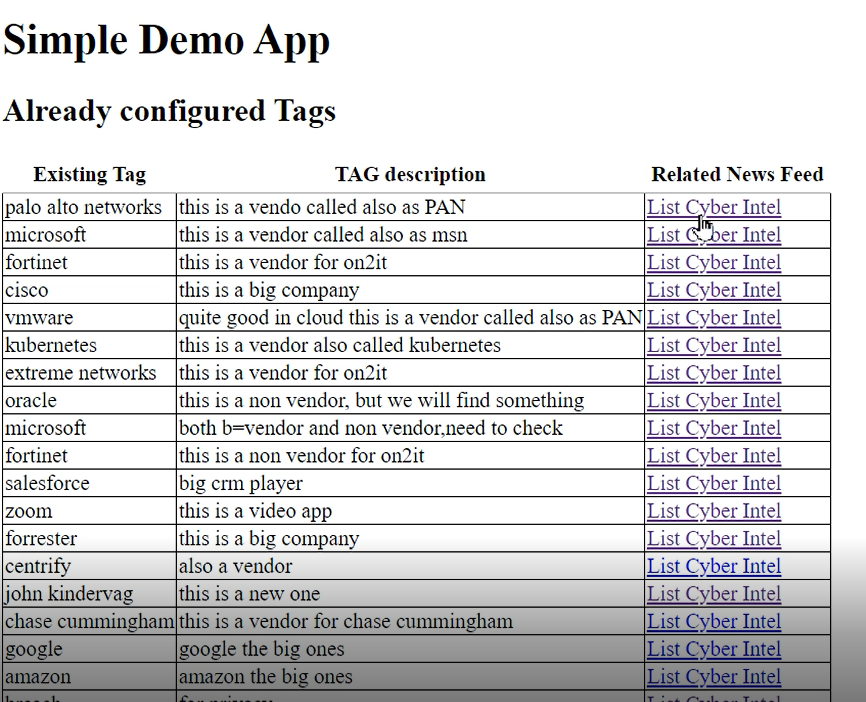
\includegraphics[width=1\linewidth]{Figures/Configured-tags.PNG}}
    \caption{Screenshot of the artefact: List of TAGs}
    \label{fig:Configured-tags}
\end{figure}
 \FloatBarrier

After tagging and filteration steps, 
our newsfeed is ready for correlation and analysis  work. The cyber newsfeeds which are not relevant are achieved and are not considered for the further processing.
We have used custom MySQL database, PHP frontend, Apache webserver and custom SQL scripts on AWS cloud to do the information processing.



In FIGURE \ref{fig:processor-rss}, we see the output as a RSS feed which can be used by a Cyber analyst for further analysis. The filter logic is mentioned in section \ref{rss-send} of Appendix \ref{AppendixChapter8}.

\begin{figure}[ht]
    \centering
   \fbox{ 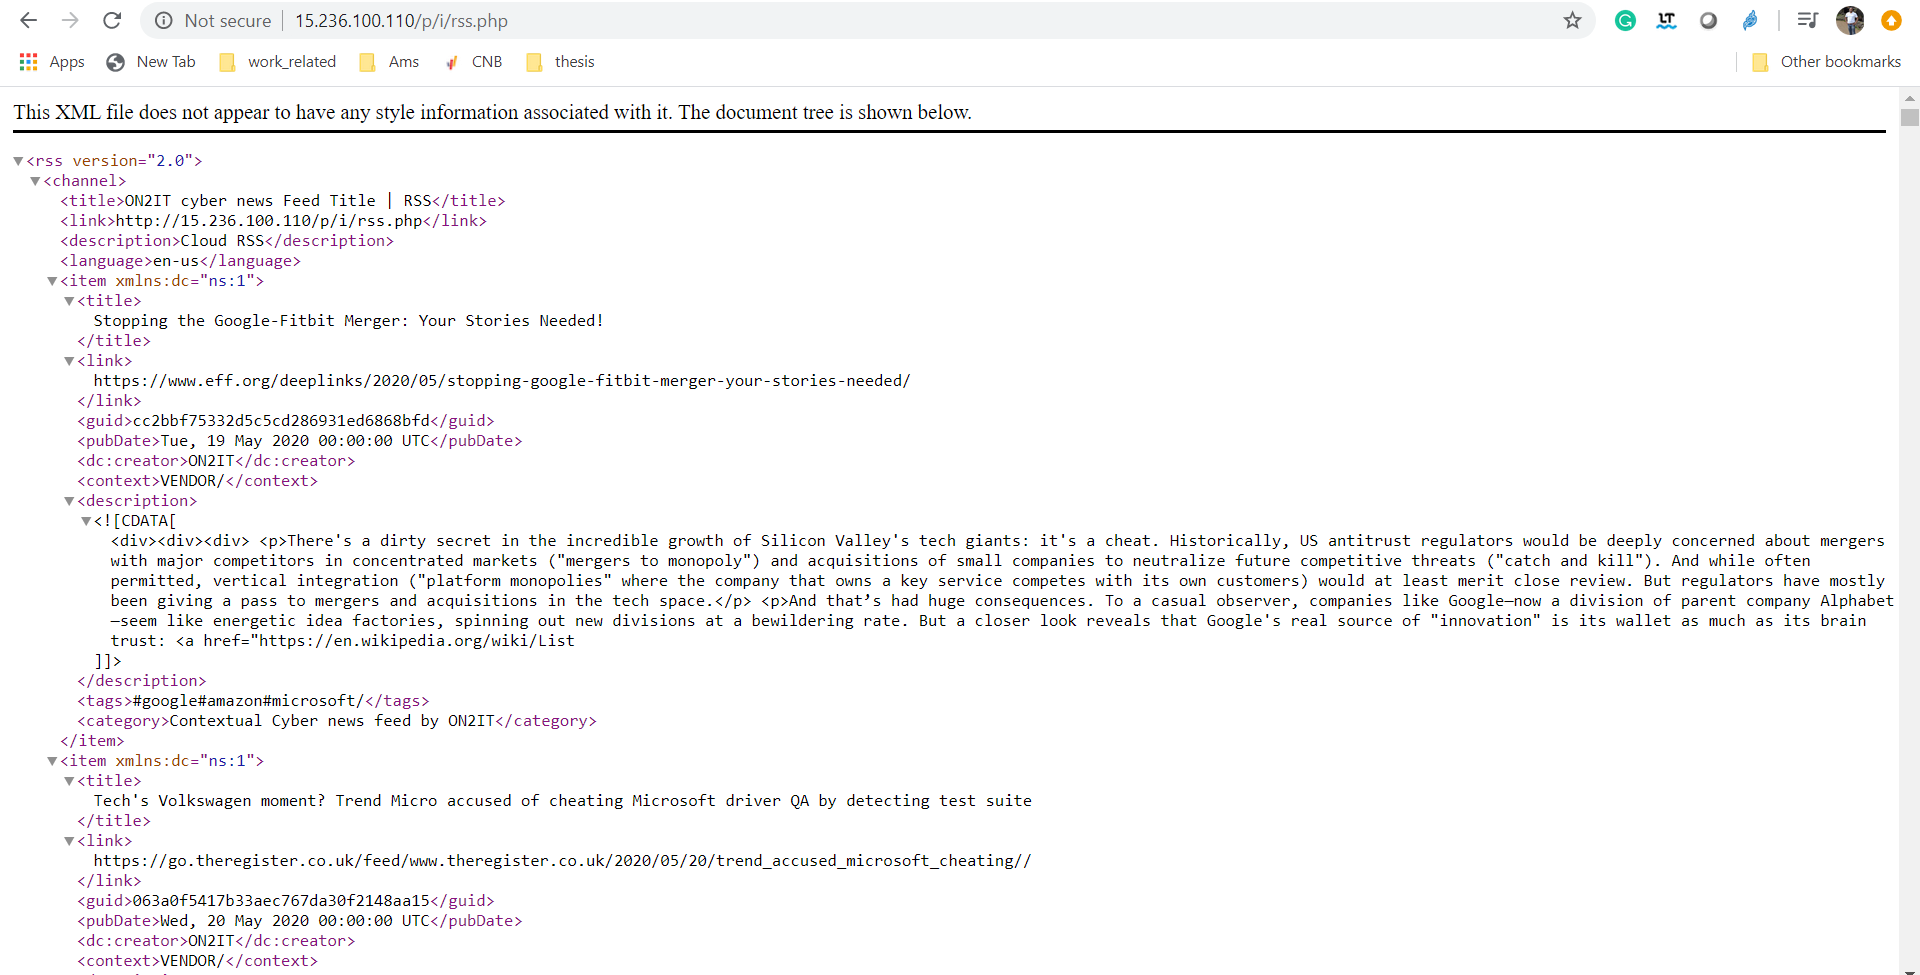
\includegraphics[width=1\linewidth]{Figures/processor-rss-output.png}}
    \caption{Screenshot of the artefact: Processor Module RSS output}
    \label{fig:processor-rss}
\end{figure}
 \FloatBarrier
\subsubsection{Analyser \& Advisory Module}
Despite having different functionality of the Analyser \& Advisory Module, I have merged the two functionalities 1) Analyser and 2) Advisory into a single module. This is done because both the modules are human dependent and it is assumed that the cyber analysts will do the Analysis and Advisory activities using the same GUI. The Analyser \& Advisory module is a mix of automatic and manual work as depicted in  FIGURE \ref{fig:analyser-advisor}

\begin{figure}[ht]
    \centering
    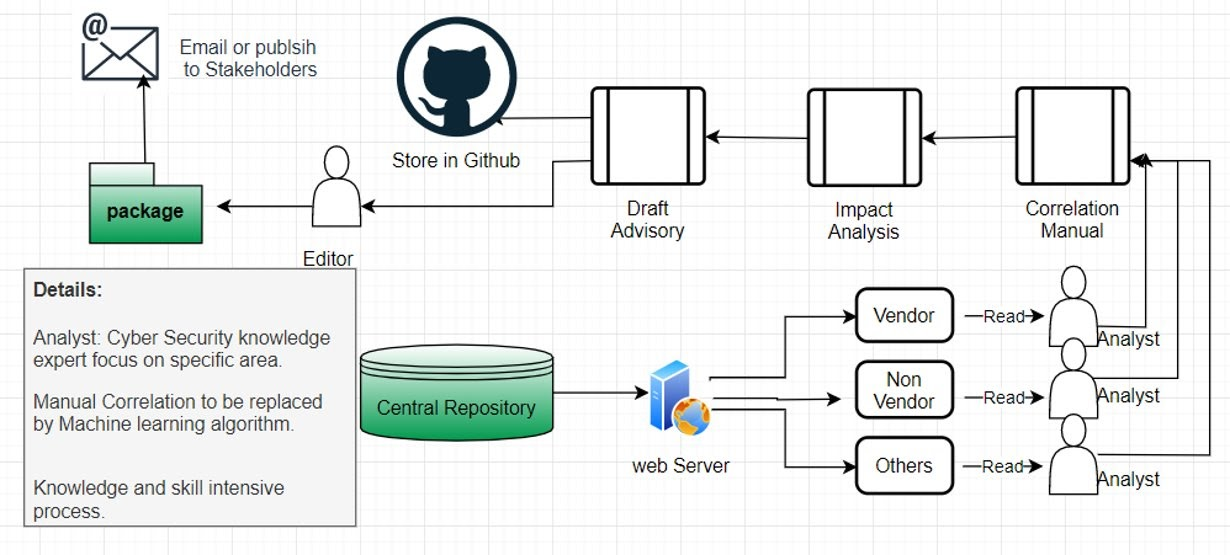
\includegraphics[width=1\linewidth]{Figures/analyser-advisor.png}
    \caption{Analyser \& Advisory Module design}
    \label{fig:analyser-advisor}
\end{figure}
 \FloatBarrier
 
 As shown in FIGURE \ref{fig:tag-intel}, 
 the cyber analysts can use the web interface of Analyser \& Advisory module 
 to find the related cyber newsfeed info.
 The cyber analysts can refer to the related cyber newsfeed data 
 and after doing their research can add advisory for the organisation-specific cyber newsfeed topic 
 as depicted in FIGURE 
 \ref{fig:add-advisory}. 
 
\begin{figure}[ht]
    \centering
    \fbox{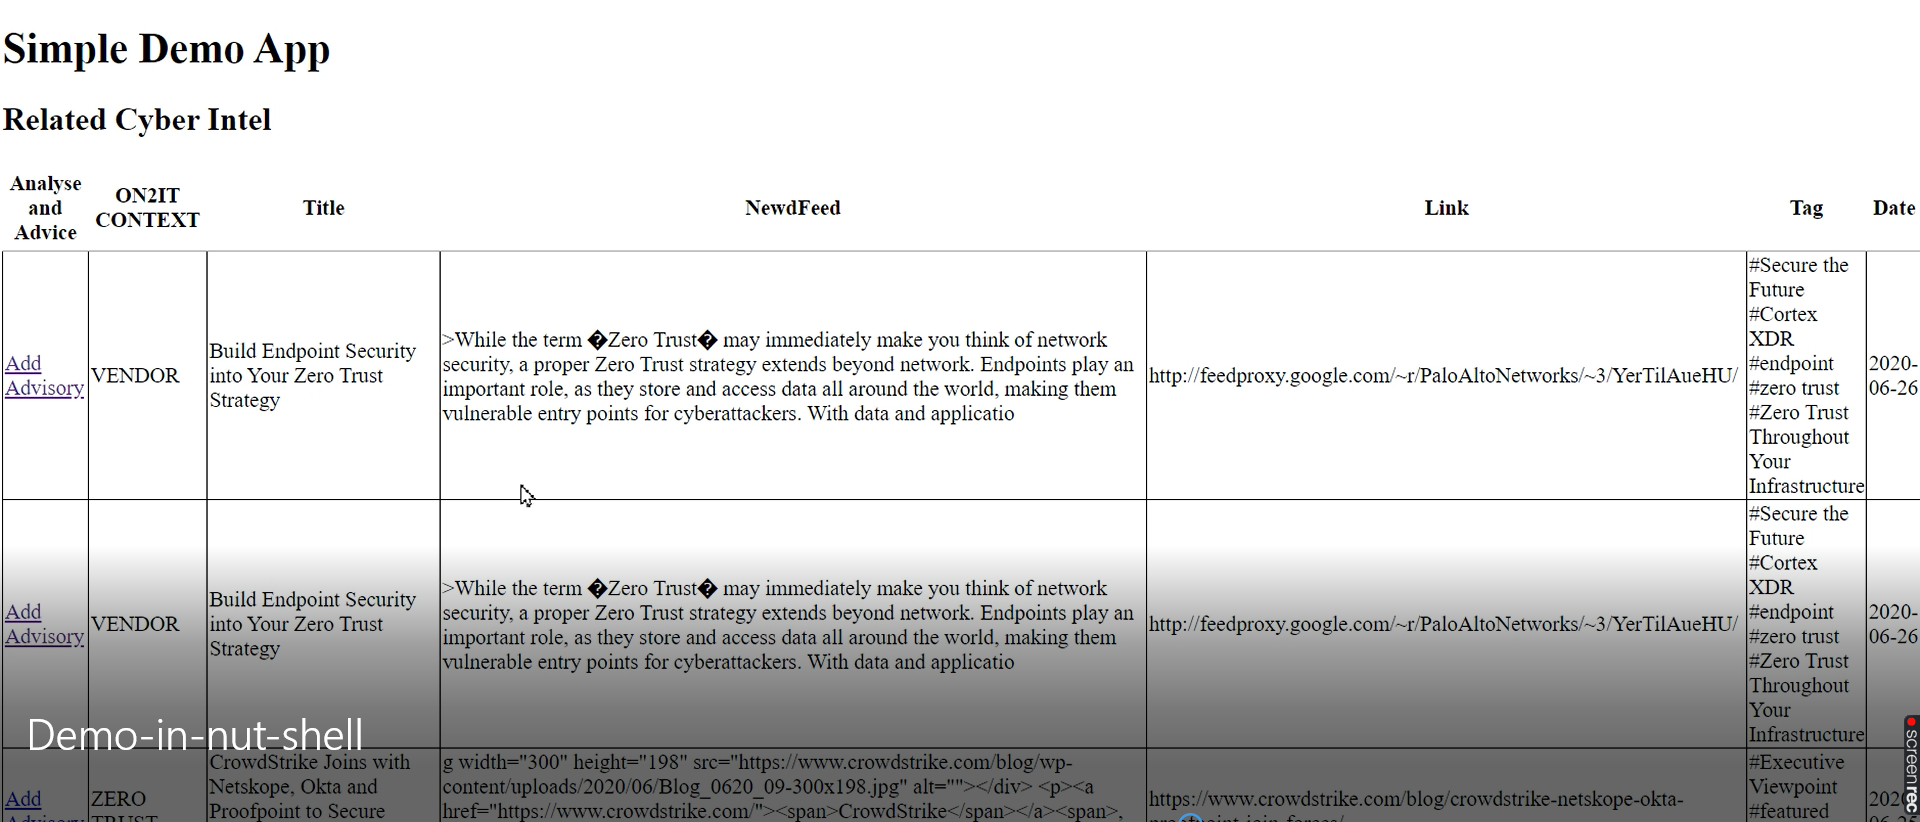
\includegraphics[width=1\linewidth]{Figures/tag-intel.PNG}}
    \caption{Screenshot of the artefact: List of co-related news}
    \label{fig:tag-intel}
\end{figure}
 \FloatBarrier
 
 

An analyst can co-relate similar cyber newsfeed items, 
he can perform impact analysis and root cause analysis for the cyber newsfeed item, which is manual. 
Finally he can add all his work and can add available solution to the cyber newsfeed items as a draft advisory as depicted in FIGURE \ref{fig:add-advisory}.

\begin{figure}[ht]
    \centering
    \fbox{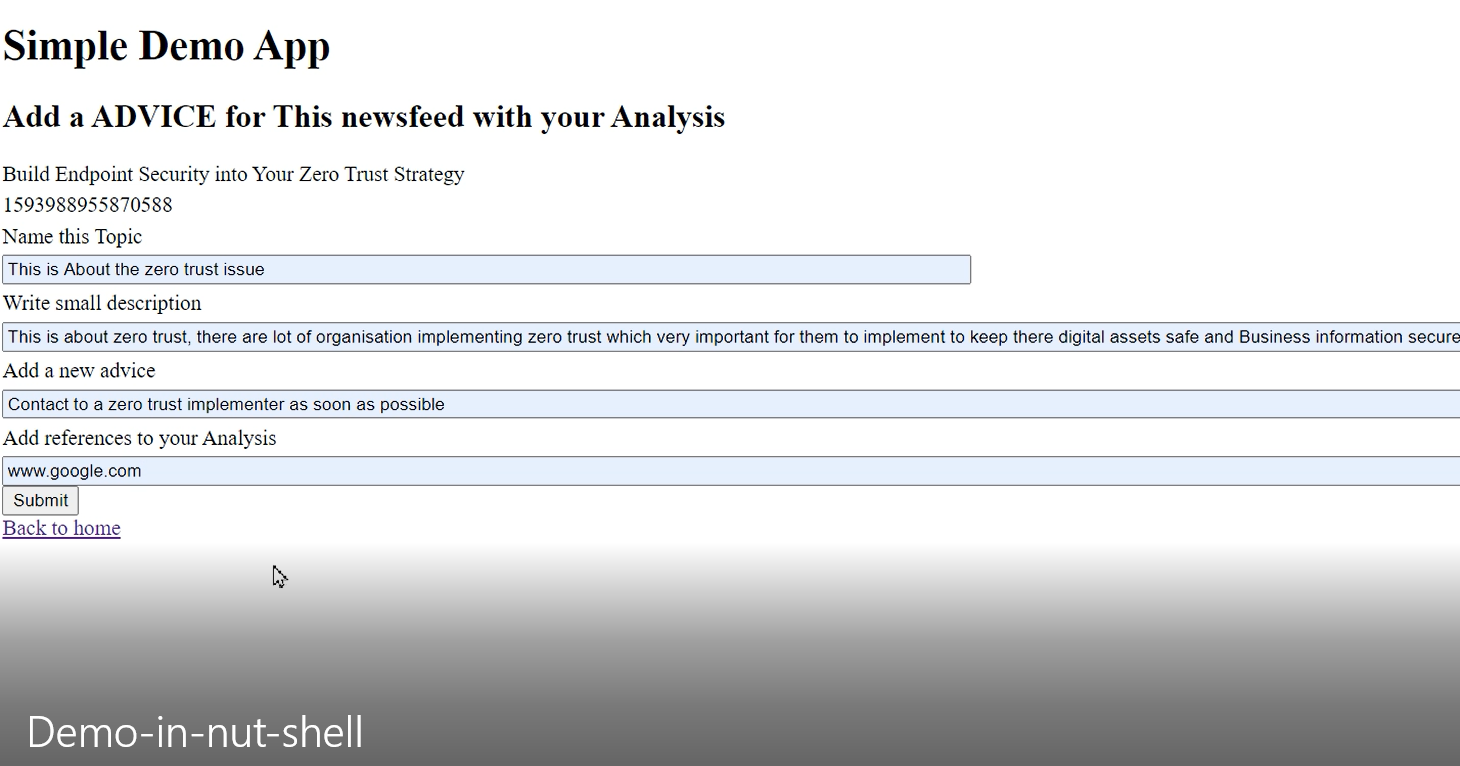
\includegraphics[width=1\linewidth]{Figures/add-advisory.PNG}}
    \caption{Screenshot of the artefact: Demo GUI to add Advisory}
    \label{fig:add-advisory}
\end{figure}
 \FloatBarrier


After analysis and adding advisory of an organisation-specific cyber newsfeeds, 
the cyber analysts can refer to the list of cyber newsfeeds Intels along with advisory being created as 
as shown in FIGURE \ref{fig:analyst-advisory-demo} and store them in the  GitHub repository for editorial validations. After editorial validations, the organisational-specific contextula cyber intels can be delivered to the stakeholders.

 
\begin{figure}[ht]
    \centering
    \fbox{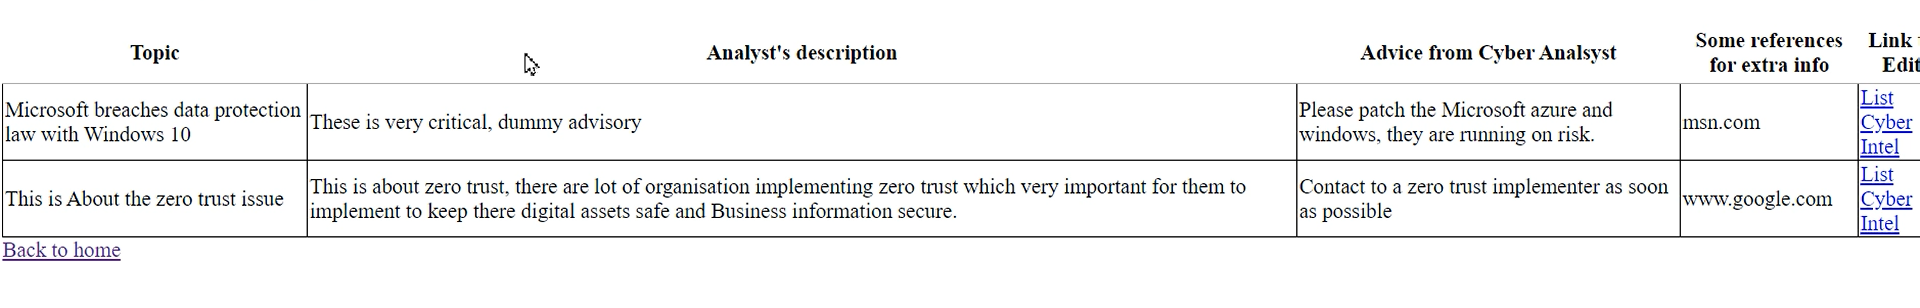
\includegraphics[width=1\linewidth]{Figures/analyst-advisory-demo.PNG}}
    \caption{Screenshot of the artefact: Demo GUI to List cyber newsfeed Intel}
    \label{fig:analyst-advisory-demo}
\end{figure}
 \FloatBarrier

Analyser \& Advisory Module helped to make the cyber newsfeed brief \footnote{A group or list of cyber news items}, which is a deliverable Intel for the stakeholders. 
The stakeholders receives the organisation-specific  context which the cyber analyst configured during the activities described in the Processor module. 

\subsection{Prototype on accessing the data source quality}
\label{quality_source}
For assessment of data sources I proposed to use one of the quantitative metrics listed in chapter  
\ref{Chapter7_literature-review}
TABLE \ref{table:quantitative}.
One of the metrics called \enquote{Extensiveness} was selected to be   implemented for this artefact because this parameter was first in the sequence. The complete formula and description for \enquote{Extensiveness} is mentioned in TABLE  \ref{table:source-quality}. 

The formula \textbf{extensiveness parameter} $p_1$ evaluates the number of extra parameters which are filled in for a Really Simple Syndication (RSS)\footnote{\url{https://validator.w3.org/feed/docs/rss2.html} } feed. 
\textbf{Symbol} $o_i$
is the sum of the filled-in optional
properties in \textbf{a cyber newsfeed} i. The \textbf{ total number of
messages shared by the source} is $z$. 
Max $y_i$ 
is the \textbf{maximum number
of optional properties} defined for this specific type of message i by
 RSS feed.
%% This file contains only a table.
%% this file is included into Chapter8

\begin{table}[htbp!]
   \setlength{\arrayrulewidth}{0.1mm}
    \setlength{\tabcolsep}{5pt}
    \renewcommand{\arraystretch}{1.0}

    \centering{}
 
    \caption{Source Quality metrics: Qualitative}
    \label{table:source-quality}
    
    \begin{tabularx}{\linewidth}{| p{1.11cm}|p{2.50cm}|p{4cm}|p{1.05cm}|p{3.7cm}|} 
    
%    |a|>{\columncolor[HTML]{FFFFFF}}C|C|C|
     \arrayrulecolor[HTML]{06000A}
        %% Table Body
        \hline
        \rowcolor[HTML]{5789F3} 
        \multicolumn{5}{|c|}{Quantitative based metrics} \\
        \hline
        
        \rowcolor[HTML]{ECB4E8} serial \# & Parameter type & Parameter Description & Symbol & Math Formula  \\
        \hline
 1	&	Extensiveness	&	Evaluates how many optional parameters are filled in	&	p1	&	\[p1 = \frac{1}{z}\sum\limits_{n=1}^{z}(\frac{oi}{\max y_i}) \]	\\ 
  
\hline
    \end{tabularx}

\end{table}







\section{Conclusion}
This concludes the chapter \ref{Chapter8_artefact-design} and with this,  the model of processes and activities required in the artefact prototype of \enquote{Cybernewsfeed Technology} was ready.
The steps taken and augmentations considered while designing and simulating the artefact on AWS cloud with the help of MySQL, Apache and PHP was also mentioned.
After the creation of this artefact the next research step is the evaluation of the artefact which is presented in next chapter.






